\documentclass[main.tex]{subfiles}
\begin{document}

\chapter*{Bilag 1 - Om Dysfagi}
\label{Bilag1}
\section*{Indledning}
Når man drikker eller spiser, passerer det indtaget bolus i mundhulen forbi svælget og videre ned i spiserøret. Denne synkesprocess foregår ved at bolus skubbes bagud mod svælget, ved hjælp af tungen som presser op og bagud. Derefter udløses en refleks pga. sanseceller i svælget. Dette foregår uden for viljens kontrol og i sammenspil med den forlængede rygmarv. Hele synkeprocessen er et samspil mellem 20-30 muskler som enten skal trække sig sammen eller slappe af i den rigtige rækkefølge \cite{Sand2008MennesketsFysiologi}. 

Synkeprocessen består af tre sammenhængende faser:
\begin{enumerate}
\item Pre Oral fase\\
Inden vi indtager føde, 
\item Oral fase (i munden)\\
I den første fase bliver maden bidt i stykker og ført i munden. Nu tykkes maden som bliver blandet med spyt og formet til en bolle (bolus). Ved hjælp af tungen transporteres bolus til den bagerste del af mundhulen samtidig med at ganespejlet lukker af op til næsen.
\item Faryngeale Fase (i svælget)\\
Nu kommer maden fra mundhulen og ned i svælget, ved at der synkes. 
\item Esophageal Fase (i spiserøret)\cite{Bass1992Dysphagia:Management}
\end{enumerate}

\begin{figure}[H]
\centering
{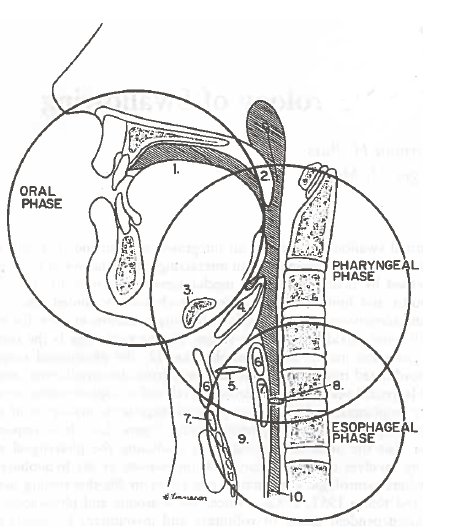
\includegraphics[width=6cm]
{Figure/dysfagi3faser}}
\caption{De tre faser ved synkeprocessen\cite{Bass1992Dysphagia:Management}}
\label{trefaser}
\end{figure}


\section*{Hvad er dysfagi?}
Dysfagi er den medicinskes betegnelse for symptom relateret til dysfunktion af synkeprocessen \cite{KjaersgaardPh.d.studerendeDYSFAGIKonsekvenser}. Dysfagi tilstanden er karakteriseret ved spise- og drikkevanskeligheder hos patienten. Resultatet kan være en fejlsynkning, ved at bolus ender i luftrøret i stedet for spiserøret. Dette kan medføre udvikling af bl.a. lungebetændelse. Dysfagi symptomerne kan observeres hos sklerose, apopleksi eller parkinson patienter. Dog forekommer symptomerne også ved kræft, KOL eller almen svækkelse og aldring\cite{SallyRefsgaardTinesterbyKristensen2015DysfagiKommune}.

Dysfagi kan have følgende konsekvenser\cite[s. 12]{KjaersgaardPh.d.studerendeDYSFAGIKonsekvenser}:
\begin{itemize}
\item Manglende oral ernæring og dermed under- eller fejlernæring
\item Dehydrering
\item Aspiration
\item Kvælning
\item Udvikling af aspirationspneumoni
\item Social isolering
\item Øget risiko for mortalitet
\item Reduceret livskvalitet

\end{itemize}



\section*{Diagnosticering af dysfagi}


Diagnosticering af øvre dysfagi kan inddeles i en tre-delt model. Den første intervention handler om at screene patientens mentale tilstand ved at vurdere patientens bevidsthedsniveau, orienteringsevne, handlekraft, samt evnen til at synke få konsistenstyper som vand og spytflåd. Hvis det vurderes af klinikeren at der er behov for yderligere udredning, sendes patienten videre til en klinisk undersøgelse. Den kliniske undersøgelse er baseret på Facial-Oral-Tract-Therapy (F.O.T.T) metoden og anvendes til at vurdere parametre som patientens sensoriske/motoriske respons, åndedræt og oral indtagelse af fødebolus \cite[s. 23-25]{Kjaersgaard2013DifficultiesPerspective}. 

Den kliniske undersøgelse er en subjektiv undersøgelse, da det foretages af en klinikker uden hjælp af teknologiske apparater. Denne undersøgelsesmetode mangler præcision til f.eks. at opdage silent aspiration, som kan medføre udvikling af lungebetændelse og i værste fald kvælning. Derfor anbefales det af sundhedsstyrelsens nationale kliniske retningslinjer for øvre dysfagi at man supplere den kliniske undersøgelse med en instrumentel undersøgelse til voksne med synkebesvær \cite{Sundhedsstyrelsen2015NationalDysfagi}.

Den instrumentelle undersøgelse omfatter Fiber Endoskopisk Evaluering af Synkefunktionen (FEES) og/eller Funktionel Videoradiologisk Evaluering af Synkefunktionen (FVES).  Ved FEES undersøgelse, som er en invasiv intervention, fører klinikeren en fiberoptisk endoskop gennem patientens næse og pharynx for at få et visuelt billede af pharynx anatomi. Anormaliteter, som observeres undervejs dokumenteres i en modificeret udgave af ”Der Berliner Dysphagia Index” som er en standard protokol til dokumentation af FEES undersøgelse \cite{afLambertsenKMDKock-JensenCMDKjrsgaardAMScOTHansenTSMsci/MPHWestergaardLMD2007ModificeretIndex}. 

Undersøgelsen kan afdække patientens synkevanskeligheder ved at iagttage aspiration af bolus i luftvejene, tilstedeværelsen af bolus-rester i strubehovedet og patientens evne til at synke egen saliva \cite[s. 27-28]{Kjaersgaard2013DifficultiesPerspective}. 
Ved FVES undersøgelse anvendes røntgenstråler, som muliggør visualisering af fødebolus i alle faser. Klinikeren kan vha. denne metode evaluere om pharyngeal eller esophageal muskler fungerer korrekt og om patienten kan kompensere for dysfagien med reflektoriske teknikker som ændring af hovedstilling. FEES og FVES anvendes som ”guld standarder” ved diagnosticering af patienter med øvre dysfagi, og begge undersøgelsesmetoder betragtes som komplementære værktøjer til udredning af dysfagi frem for konkurrerende \cite[s. 50]{Kjaersgaard2013DifficultiesPerspective}.



\bibliography{Mendeley.bib}
\end{document}